\documentclass[a4paper,10pt, twoside]{report}
\usepackage[utf8x]{inputenc}
\usepackage[T1]{fontenc}
\usepackage{titlesec, blindtext, color}
\usepackage{setspace}

\usepackage[hidelinks]{hyperref}

\usepackage[export]{adjustbox}
\usepackage{array}
\usepackage{color, colortbl}

\usepackage{float}
\usepackage{fancyhdr}
\usepackage{graphicx}
\usepackage[top=2cm, bottom=3cm, left=2.5cm, right=2.5cm]{geometry}

\usepackage[french]{babel}

% page style
\pagestyle{fancy}
\setlength{\headheight}{49pt}
\setlength{\footskip}{17pt}

% header
\fancyhead[R]{
\includegraphics[width=5cm]{logo_sciences.png}}
\fancyhead[L]{
\includegraphics[width=5cm]{logo_arksens.png}}

% footer
\fancyfoot[C]{Rapport de stage --- Master 2 FSIL\\Ludovic Lubeigt}
\fancyfoot[RO, LE] {\thepage}

% colors
\definecolor{gray73}{gray}{0.73}
\definecolor{arkred}{rgb}{0.592, 0.145, 0.168}

% commands
\newcommand{\hsp}{\hspace{20pt}}
\titleformat{\chapter}[hang]{\Huge\bfseries}
{\thechapter\hsp\textcolor{gray73}{|}\hsp}{0pt}{\Huge\bfseries}
\titleformat{\subsubsection}{}{}{}{\textbullet~}

\graphicspath{{images/}}

\begin{document}
\begin{spacing}{1.2}
 
% Page de garde
\begin{titlepage}
  \newgeometry{top=2cm, bottom=2cm, left=2cm, right=2cm}
  
  \begin{center}
    
\includegraphics[width=9cm]{logo_sciences.png}\\[2cm]
    
    \textsc{\bfseries\Large Rapport de stage\\[0.3cm]
    Master 2 -- Fiabilit\'e, S\'ecurit\'e et
    Int\'egration Logicielle\\[0.3cm]
        Parcours Fiabilit\'e et S\'ecurit\'e Informatique}\\[0.3cm]

    \rule{\linewidth}{1mm} \\[1cm]

    \textsc{\bfseries\huge Conception \&  d\'eveloppement syst\`eme de backup
    chiffr\'e et incr\'emental en C/C++}\\[1cm]

    \rule{\linewidth}{1mm}\\[1.5cm]

    \textsc{\huge Arksens Cyber Security}\\[2cm]
    
    \begin{figure}[H]
      \begin{minipage}[t]{8cm}
        \centering
        
\includegraphics[scale=0.50]{logo_adhara.png}
      \end{minipage}
      \begin{minipage}[t]{8cm}
        \centering
        
\includegraphics[width=7cm]{logo_arksens.png}
      \end{minipage}\\[1.3cm]
    \end{figure}
      
    \begin{minipage}{0.4\textwidth}
      \begin{flushleft} \large
        \emph{\bfseries Auteur :}\\
        Ludovic \textsc{Lubeigt}
      \end{flushleft}
    \end{minipage}
    \begin{minipage}{0.4\textwidth}
      \begin{flushright}
        \large \emph{\bfseries Tuteur Entreprise :}\\
        Ga\"etan \textsc{van Diemen}\\[0.2cm]
        \emph{\bfseries Enseignant :}\\
        Jean-Luc \textsc{Massat}
      \end{flushright}
    \end{minipage}\\[1.5cm]
      
    \large\emph{\bfseries Ann\'ee Universitaire :}\\
    2014 -- 2015

  \end{center}
\end{titlepage}

\begin{abstract}

Ce document pr\'esente le travail r\'ealis\'e lors du stage de fin d'\'etude
\`a Arksens Ltd. \`a l'\^ile Maurice entre le premier avril 2015 et le 25
septembre 2015 dans le cadre du Master 2 Fiabilit\'e et S\'ecurit\'e
Informatique \`a l'Universit\'e d'Aix-Marseille.

Le rapport est d\'ecoup\'e en deux parties. Une premi\`ere servant de rapport
de synth\`ese et pr\'esentant l'entreprise, le sujet de stage, le
travail effectu\'e de m\^eme que l'environnement de travail et les \'eventuelles
difficult\'es rencontr\'ees.
La seconde partie apporte un aspect technique au rapport et permet de 
pr\'esenter le travail r\'ealis\'e plus en d\'etail.
\end{abstract}

\newpage
\hfill
\section*{Remerciements}
Je tiens tout d'abord \`a remercier l'\'equipe p\'edagogique de la facult\'e des
sciences de l'universit\'e d'Aix-Marseille qui m'a permis d'avoir les
connaissances et les aptitudes n\'ecessaires au bon d\'eroulement de ce stage.

Je remercie \'egalement la soci\'et\'e Arksens pour m'avoir permis de faire mon
stage chez eux. Tout particuli\`erement, je remercie David Terranova et Ga\"etan
van Diemen qui m'ont accueilli \`a l'\^ile Maurice et suivi au jour le jour
durant ces six mois. Je n'oublie \'evidemment pas Micha\"el Colaone et le reste
de l'\'equipe pour l'accueil et la bonne ambiance au sein de l'entreprise.

Enfin je remercie toute les personnes que je peux oublier mais qui m'ont aid\'e,
dans l'\'ecriture de ce rapport, dans le cadre du stage ou qui m'ont tout
simplement fait d\'ecouvrir l'\^ile Maurice.

Je tiens tout particuli\`erement \`a remercier Sir Daniel Brands of House Brands,
the first of His Name, King of the Dutch, King of the flatlands and the first
Men, Breaker of Cars and Father of the Bikers.

\hfill
\tableofcontents
\thispagestyle{fancy}

\chapter*{Introduction}
\thispagestyle{fancy}
Dans le cadre du Master professionnel \textit{Fiabilit\'e, S\'ecurit\'e et
Int\'egration logicielle}, parcours \textit{Fiabilit\'e et S\'ecurit\'e
Informatique} \`a l'\textit{Universit\'e d'Aix-Marseille}, un stage de fin
d'\'etude doit \^etre effectu\'e en entreprise pour valider les acquis et
rentrer dans le monde professionnel.

J'ai r\'ealis\'e ce stage entre le 1\up{er} avril et le 25 septembre 2015, soit
une p\'eriode de six mois, dans l'entreprise \textit{Adhara Cyber Security},
renomm\'ee \textit{Arksens} au 1\up{er} juillet.

Ce stage fut donc l'occasion pour moi de mettre en pratique mes connaissances,
acquises tout au long de mon parcours universitaire, dans un environnement
professionnel et de m'en servir pour mener au mieux la mission qui m'a
\'et\'e confi\'ee. Ma mission, durant ce stage, a \'et\'e de concevoir et
d\'ev\'elopper un syst\`eme de backup incr\'ementale et s\'ecuris\'e, offrant
une encryption en local des donn\'ees des utilisateurs. J'ai ainsi proc\'ed\'e
\`a la r\'edaction du plan de d\'eveloppement puis \`a l'impl\'ementation de
celui-ci, et j'ai ainsi particip\'e au processus de cr\'eation, jusqu'\`a un
stade avanc\'e, de ce qui peut \^etre qualifi\'e de gros projet.

Ce rapport pr\'esente donc le d\'eroulement du stage ainsi que le travail
accompli au sein de l'entreprise durant ces six mois.


\chapter{Rapport de synth\`ese}
\thispagestyle{fancy}
\label{rapportSynthese}
\section{Pr\'esentation de l'entreprise}
Cr\'e\'ee en 2013 sous le nom d'\textit{Adhara Cyber Security} avant
d'\^etre renomm\'ee \textit{Arksens} au 1\up{er} juillet 2015, l'entreprise 
dans laquelle j'ai effectu\'e mon stage est sp\'ecialis\'ee en s\'ecurit\'e
informatique. L'entreprise se d\'eveloppe sur trois continents gr\^ace \`a une
approche novatrice et r\'epondant aux besoins des entreprises et
administrations de toutes tailles.

Le changement de nom a fait suite \`a une \'evolution des clients puisque
l'entreprise, bien que principalement prestataire de service pour des PME
s'est ouverte aux entreprises de taille plus importante. Revoyant leur
strat\'egie de commercialisation et de communication, l'entreprise se devait
donc de changer de nom.

\subsection{Pr\'esence dans le monde}
Aujourd'hui \textit{Arksens} est donc pr\'esent dans trois pays chacun sur
un continent diff\'erent (voir figure~\ref{mapArksens}) offrant ainsi aux
utilisateurs un service de proximit\'e :
\begin{itemize}
  \item Abu Dhabi aux \'Emirats Arabes Unis pour les activit\'es au Moyen
  Orient.
  \item Pamplemousses à l’\^ile Maurice pour les activit\'es africaines.
  \item Paris en France pour les activit\'es européennes.
\end{itemize}

\begin{figure}[h!]
  \centering
  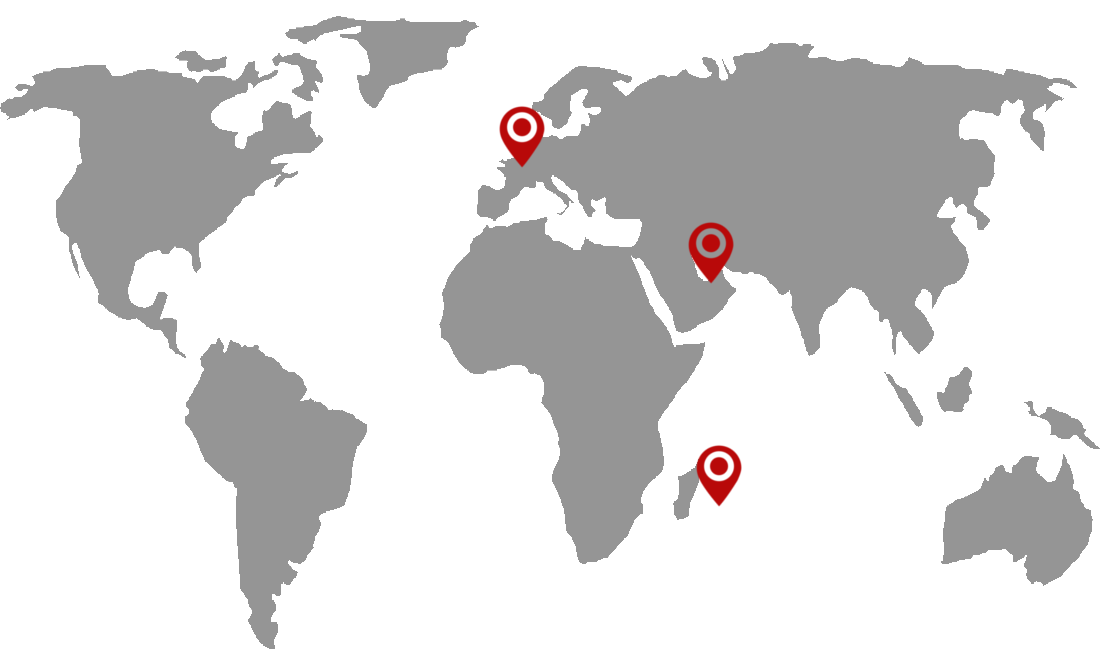
\includegraphics[scale=0.30]{map_arksens.png}
  \caption{\label{mapArksens} O\`u trouver Arksens}
\end{figure}
      
\subsection{Produits et solutions}
\textit{Arksens} propose aux entreprises 6 produits et solutions autour de la
s\'ecurit\'e informatique. Une rapide description de ces produits se trouve
table~\ref{tabProduits} :
\begin{table}[h!]
  \centering
  \def\arraystretch{1.5}
  \setlength{\fboxsep}{13pt} % padding
  \setlength{\fboxrule}{0pt} % frame
  \begin{tabular}{m{6cm}m{6cm}}
   \rowcolor{arkred} 
    \arrayrulecolor{gray73}\hline
    \color{white} \textbf{Produit} & \color{white} \textbf{Description} \\
    
\includegraphics[width=5cm, fbox]{produits/mail.png} & Prot\'eger l'information
    transitant par les mails. H\'ebergement de serveur email s\'ecuris\'e dans
    un cloud d\'edi\'e.\\
    \hline
    
\includegraphics[width=5cm, fbox]{produits/whisper.png} & Communications voix
    et images s\'ecuris\'es et anonymes.\\
    \hline
    
\includegraphics[width=5cm, fbox]{produits/backup.png} & Syst\`eme de
    chiffrement et de sauvegarde des donn\'ees dans un cloud d\'edi\'e.\\
    \hline
    
\includegraphics[width=5cm, fbox]{produits/gateway.png} & S\'ecuriser et
    rendre anonyme la navigation sur internet.\\
    \hline
    
\includegraphics[width=5cm, fbox]{produits/endpoint.png} & S\'ecuriser les
    postes utilisateurs en locales. C'est une ligne de d\'efense pour palier
    \`a la diffusion d'\'eventuels logiciels malveillants (virus, chevaux de
    Troie, vers, logiciels espions,\ldots{}) sur les ordinateurs et les
    serveurs.\\
    \hline
    
\includegraphics[width=5cm, fbox]{produits/nomad.png} & S\'ecuriser les
    donn\'ees personnelles sur appareils mobiles.\\
    \hline
  \end{tabular}
  \caption{\label{tabProduits} Produits et solutions par \textit{Arksens}}
\end{table}

L'ensemble des produits et solutions propos\'es par l'entreprise sont d\'ecrit
de mani\`ere plus compl\`ete sur leur site web~\cite{refArksens}.

\subsubsection{Les offres de cloud}
L'entreprise propose \'egalement des offres autour du Cloud\footnote{
Exploitation de la puissance de calcul ou de stockage de serveurs distants
par l'interm\'ediaire d'un r\'eseau, g\'en\'eralement l'internet.}

\begin{itemize}
  \item Offre 1 - Pure cloud
  \noindent
  \begin{itemize}
    \item 100 \% des services sont h\'eberg\'es
    \item La gestion est assur\'ee par \textit{Arksens}
    \item Des fonctionnalit\'es suppl\'ementaires sont propos\'ees telles que
    l'h\'ebergement de fichiers ou de logiciels
  \end{itemize}
  \item Offre 2 - Hybrid cloud
  \noindent
  \begin{itemize}
    \item Un h\'ebergement local avec une ``box'' chifr\'ee et une
    r\'eplication sur le cloud \textit{Arksens}
    \item La gestion est assur\'ee par \textit{Arksens}
    \item Id\'eal pour les clients souhaitant une r\'eplication dans leurs
    locaux
  \end{itemize}
  \item Offre 3 - Private cloud
  \noindent
  \begin{itemize}
    \item Le cloud est pr\'esent uniquement chez le client dans une salle de
    serveurs ou dans un centre de donn\'ees
    \item La gestion est assur\'ee par \textit{Arksens}
    \item Id\'eal pour les clients souhaitant stocker l'ensemble des services
    et des donn\'ees localement (comme les banques, la d\'efense,
    l'audit\ldots{})
  \end{itemize}
\end{itemize}

Avec 3 offres de cloud comportant l'ensemble des solutions de s\'ecurit\'e
cité pr\'ec\'edemment, \textit{Arksens} peut répondre à l'ensemble des besoins
de ses clients actuels.

\subsection{L'id\'eologie de l'entreprise}
\subsubsection{La politique des centres de données}

Pour chaque service, \textit{Arksens} fournit le mat\'eriel (centres de
donn\'ees), le produit et le support qui va avec. Pour \^etre en mesure de
fournir les meilleurs services, elle poss\`ede une politique de s\'election des
centres de donn\'ees qu'elle utilise. Ci-dessous une liste repr\'esentant les
diff\'erents aspects les plus importants que doivent respecter les centres de
donn\'ees :

\begin{itemize}
  \item Uniquement des Tier IV (Haute disponibilit\'e\footnote{Mesure de
  performance. C'est le temps durant lequel le syst\`eme est op\'erationnel par
  rapport \`a sa dur\'ee totale d'exploitation} : 99,995 \%)
  \item Toutes les données sont chiffr\'ees sur les serveurs d\'edi\'es
  \item Les centres de donn\'ees doivent se situés dans des pays libres
  respectant le \textit{Patriot Act}~\cite{refPatriotAct}
\end{itemize}

De ce fait l'entreprise a actuellement des centres de donn\'ees en France
chez OVH~\cite{refOVH} qui lui conf\`ere en plus une solution contre les
attaques DDoS\footnote{Attaque par d\'eni de service. Le principe est d'envoyer
une multitude de requ\^ete depuis plusieurs sources diff\'erentes pour rendre
un service indisponible.} et en Suisse chez AlpineDC~\cite{refAlpineDC} dont la
l\'egislation est une des plus restrictive en mati\`ere de protection de
donn\'ees personnelles.

\subsubsection{La culture Open Source}

L'open source est une tradition dans l'entreprise. L'ensemble des
produits respectent les crit\`eres \'etablis par l'Open Source
Initiative~\cite{refOSI}, \`a savoir :

\begin{itemize}
  \item Possibilit\'e de redistribution
  \item Accès au code source
  \item Cr\'eation de travaux d\'eériv\'eés
\end{itemize}

Ce choix permet notamment d'accentuer la confiance avec les clients et
d'am\'eliorer le niveau de s\'ecurit\'e des produits gr\^ace aux avantages
suivants :

\begin{itemize}
  \item Logiciel ind\'ependant : aucune porte d\'erob\'ee
  (\textit{backdoor})\footnote{Fonctionnalit\'e inconnue de l'utilisateur
  l\'egitime et qui donne un acc\`es secret au logiciel} ne peut
  \^etre introduite par une organisation externe puisque les produits sont
  d\'evelopp\'es par \textit{Arksens} pour \textit{Arksens}
  \item Communaut\'e : l'acc\`es facile aux produits permet de cr\'eer une
  communaut\'e d'utilisateurs capable sur le long terme de proposer un
  support sur les produit d\'evelopp\'es, des am\'eliorations, mais aussi
  permet de d\'eceler des bogues
  \item Code source accessible : tout le monde a acc\`es au code source,
  rien n'est cach\'e, la cr\'edibilit\'e et la qualit\'e des produits est ainsi
  mise en avant
\end{itemize}

\subsection{\^Ile Maurice}
L'\^ile Maurice abrite es locaux accueillant le centre de recherche et
d\'eveloppement de l'entreprise. Les locaux se trouvent au Business Park de
Beau Plan (figure~\ref{beauPlan}) \`a Pamplemousses, ville situ\'ee au
nord-ouest de l'\^ile, \`a proximit\'e de Port Louis. C'est donc l\`a que
j'ai effectu\'e mon stage.

\begin{figure}[h!]
  \centering
  \includegraphics[width=15cm]{beau_plan_soir.jpg}
  \caption{\label{beauPlan} Beau Plan Business Park}
\end{figure}

L'\'equipe a beaucoup \'evolu\'ee entre mon arriv\'ee et mon d\'epart puisque
seulement trois personnes en plus du PDG, Micha\"el Colaone, \'etaient
pr\'esentent au 1\up{er} avril, date de d\'ebut du stage : David Terranova,
directeur des op\'erations, Ga\"etan van Diemen, chef de projet ainsi que
Daniel Brands, d\'eveloppeur web arriv\'e quelques jours auparavant.

L'\'equipe s'est agrandie par deux fois. D'abord \`a la mi-avril avec
l'arriv\'ee de deux autres stagiaire, Didier Mannone et
Yves Colin de Verdi\`ere, puis au 1\up{er} mai avec l'arriv\'ee d'Aymeric
Tabourin, ing\'enieur s\'ecurit\'e.

\`A mon d\'epart, une restructuration \'etait en cours et plusieurs changements
allait \^etre apport\'es au niveau de l'\'equipe en place avec notamment le
d\'epart de certains collaborateurs.

Ces changements montrent que la vie d'une startup peut rapidement \'evoluer,
que ce soit dans un sens ou dans l'autre. En l'espace de six mois seulement
une p\'eriode de recrutement s'en \'etait donc suivi d'une restructuration
importante impliquant le d\'epart de plusieurs employ\'es.

N\'eanmoins, au cours de mon passage dans l'entreprise, la pr\'esence de
Durant mon stage dans l'entreprise, la pr\'esence de collaborateurs
N\'eerlandais et Mauriciens a permis la cr\'eation d'un environnement
international, bien que fortement francophone. Afin de pouvoir communiquer avec
l'ensemble des personnes de l'\'equipe, l'utilisation de l'anglais au quotidien
\'etait donc une n\'ecessit\'e.

L'int\'egration dans l'\'equipe s'est donc faite assez facilement et rapidement
et c'est ainsi dans une ambiance g\'en\'eralement bonne, bien que quelque peu
compliqu\'ee sur la fin d\^u \`a la restructuration de l'entreprise s'est
d\'eroul\'e ce stage de fin d'\'etude.

\section{Sujet de stage}
\subsection{Contexte}
L'entreprise \'etant encore jeune et de petite taille, plusieurs des services
existant \'etaient bas\'e sur des produits open source qui avaient \'et\'e
int\'egr\'e au \textit{manager} (voir figure~\ref{managerFront}).

Ce \textit{manager} est un environnement web d\'evelopp\'e et maintenu par
\textit{Arksens}. Il permet aux utilisateurs de g\'erer les services auxquels
ils ont souscrit \`a partir d'un unique endroit, centralis\'e, et ainsi
faciliter l'utilisation de ces derniers.

\begin{figure}[h!]
  \centering
  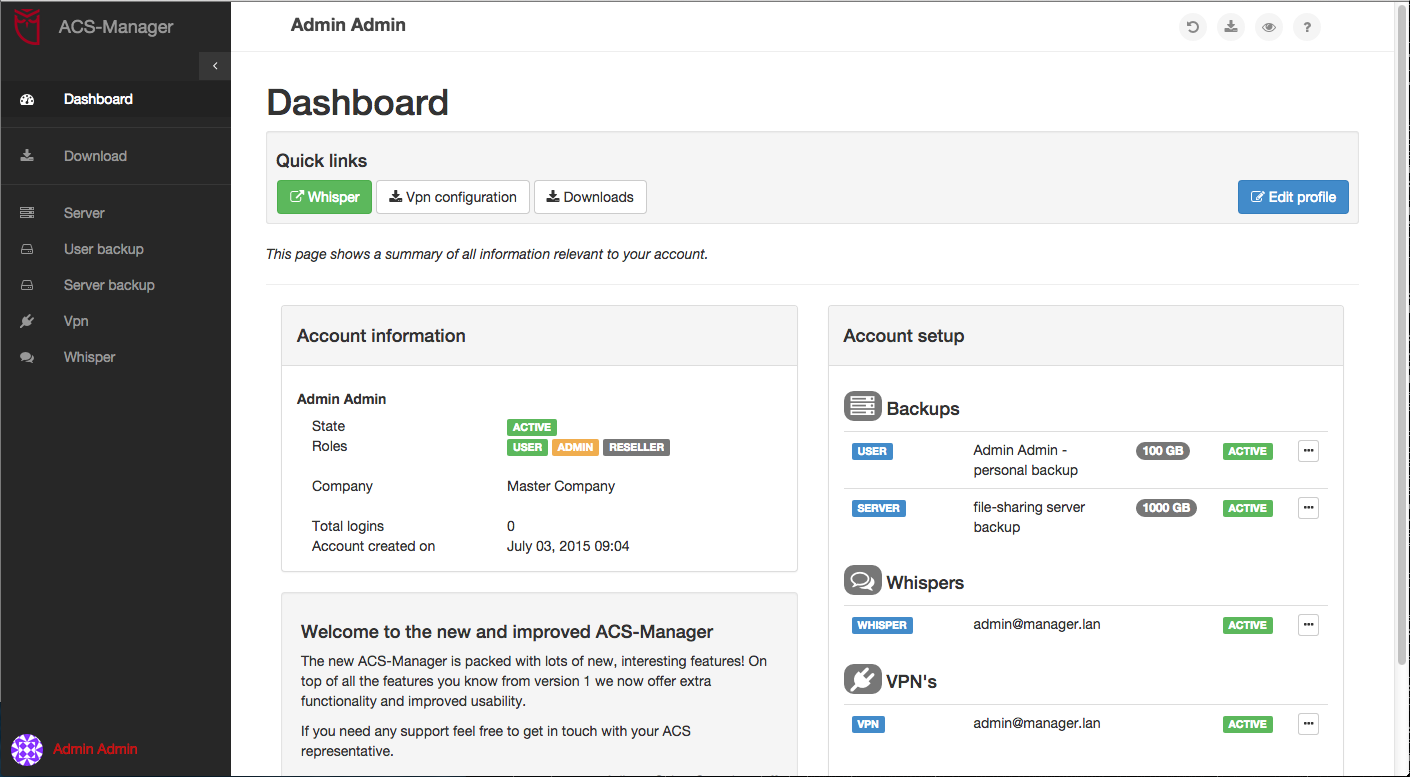
\includegraphics[width=15cm]{produits/manager.png}
  \caption{\label{managerFront} Page d'accueil du \textit{manager}}
\end{figure}

L'objectif de ce recrutement important \'etait pour l'entreprise de petit \`a
petit d\'evelopper ses propre solutions afin de proposer aux utilisateurs des
produits adapt\'es et r\'epondant \`a leurs besoins tout en minimisant
l'utilisation de logiciels tiers.

De plus les syst\`emes de backup ne sont souvent pas consid\'er\'es par les
entreprises avant qu'une perte de donn\'ees, plus ou moins importante,
ne survienne. Cons\'equences financi\`eres, temps pass\'e \`a reconstituer le
savoir \'evapor\'e ou encore impact sur la r\'eputation de l'entreprise ne sont
que des exemples de ce qui peut arriver dans une telle situation. Pour
pr\'evenir ce probl\`eme un syst\`eme de backup est non seulement n\'ecessaire
mais presque obligatoire.

Pour cela, \textit{Arksens} voulait offrir \`a ses clients un syst\`eme de
sauvegarde fiable, s\'ecuris\'e et optimis\'e afin de pouvoir \^etre
ex\'ecut\'e sur ordinateurs les moins performant. De plus la prise en compte de
connexion internet pouvant \^etre parfois tr\`es lente \'etait une
obligation. En particulier, une partie du march\'e vis\'e par \textit{Arksens}
se trouve en Afrique o\`u l'acc\`es \`a un internet rapide n'est pas toujours
aussi facile que ce qu'il peut y avoir en Europe.

C'est donc dans ce cadre que je suis arriv\'e et qu'il m'a \'et\'e demand\'e
de cr\'eer la prochaine g\'en\'eration de backup pour \textit{Arksens}.

\subsection{Le sujet}
Ma mission pour ce stage \'etait donc de faire la conception et le
d\'eveloppement d'un syst\`eme de backup incr\'emental et dont les donn\'ees
sauvegard\'ees sont chiffr\'ees en local, sur la machine client, avant d'\^etre
envoy\'ees sur des serveurs distant. Il me fallait donc d\'evelopper un
client/serveur multi-plate-forme, robuste et s\'ecuris\'e r\'epondant \`a
la probl\'ematique suivante : combiner le chiffrement local avec la sauvegarde
incr\'ementale.

Ce backup permettrait donc, au premier lancement, de sauvegarder l'ensemble
d'un ou plusieurs dossier. \`A partir de la seconde sauvegarde, il ne faudrait
n\'eanmoins sauvegarder que les changements sur les fichiers.

\`A mon arriv\'ee, David et Ga\"etan avait d\'ej\`a des id\'ees sur la
mani\`ere de r\'ealiser ce syst\`eme de sauvegarde, id\'ees que nous verrons
plus loin dans ce rapport. Et c'est \`a partir de celles-ci que j'ai pu
d\'emarrer mon travail, qui sera alors divis\'e en trois grandes phases :

\begin{itemize}
 \item Phase de documentation et de r\'eflexion sur la probl\'ematique
 \item Conception logicielle
 \item D\'eveloppement
\end{itemize}

La premi\`ere phase de documentation et de r\'eflexion consistait \`a
rechercher diff\'erentes solutions d\'ej\`a existantes et potentiellement
exploitable avant de proc\'eder \`a toute phase de conception.

La conception s'est faite en prenant en compte les contraintes existantes
et en se basant sur un travail de r\'eflexion d\'ej\`a effectu\'e par David et
Ga\"etan avant mon arriv\'ee.

Enfin, en ce qui concerne le d\'eveloppement, une des contraintes que j'avais
\'etait d'utiliser le C++ et de d\'evelopper de mani\`ere orient\'e objet tout
en faisant en sorte que le code puisse \^etre robuste, lisible, testable, et
donc facilement maintenable. De plus les librairies et framework utilis\'es
devaient \^etre sous licence libre afin d'\^etre en droit de publier l'ouvrage
sous licence libre.

Pour mener cette mission \`a bien, il avait \'et\'e d\'ecid\'e qu'une r\'eunion
hebdomadaire devait \^etre r\'ealis\'ee afin que David et Ga\"etan puissent
suivre l'avancement du projet mais aussi pour voir le travail effectu\'e la
semaine pr\'ec\'edente, essayer de r\'esoudre tout probl\`eme qui aurait pu
survenir et planifier la semaine suivante.
C'est en tout cas dans cette optique l\`a que nous avions commenc\'e. Dans les
fait, le retour des clients lors de mises \`a jour d'un produit ou des
r\'eunions avec les potentiels futur clients pouvait prendre la priorit\'e et
ainsi retarder ou annuler les r\'eunions hebdomadaire.

\section{D\'eroulement du stage}
Avant de commencer le projet en lui-m\^eme, David et Ga\"etan m'ont fait part
de leur r\'eflexion sur le possible fonctionnement du syst\`eme de sauvegarde.

\begin{figure}[h!]
    \hspace{-4.5em}
    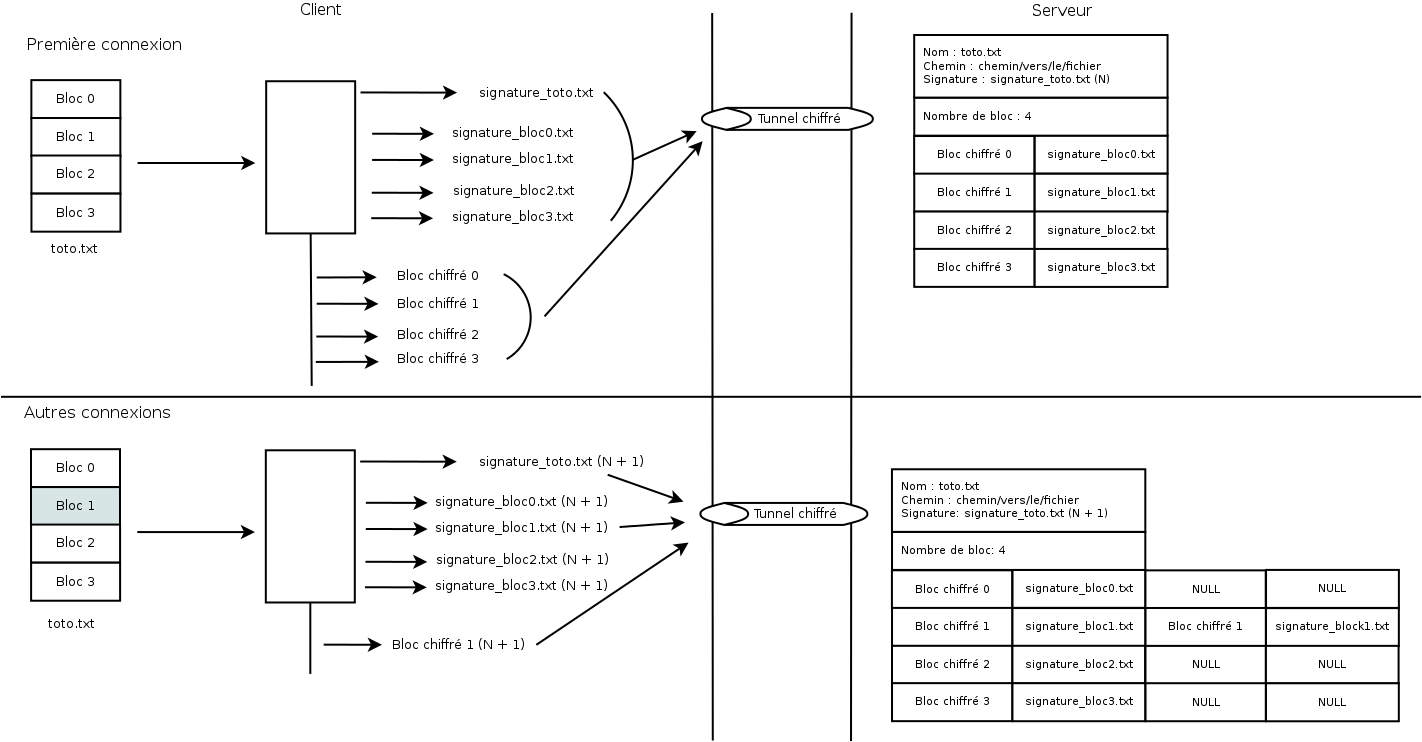
\includegraphics[width=19cm]{algo/schemaInitial.png}
    \caption{\label{schemaInitial} Sch\'ema initial du fonctionnement du backup}
\end{figure}

Le syst\`eme a deux comportement diff\'erent lors de la sauvegarde d'un fichier.
D'abord pour la premi\`ere connexion, o\`u une sauvegarde int\'egrale est
n\'ecessaire, puis lors des connexions suivantes o\`u seulement les
modifications doivent \^etre envoy\'ees.

Dans le premier cas, le fichier est d\'ecoup\'e en blocs de taille \'egale
avant d'\^etre chiffr\'e puis envoy\'e accompagn\'e des signatures calcul\'es
pour chaque bloc ainsi que pour le fichier en lui m\^eme. Les signatures
permettant de v\'erifier l'int\'egrit\'e des fichiers.

Le second cas est un peu plus complexe et d\'ecrit comme suit :
\begin{itemize}
 \item Calculer \textit{signature\_toto.txt} \`a \(N + 1\)
 \item T\'el\'echager \textit{signature\_toto.txt} \`a \(N\))
 \item Comparer les deux signatures : si elles ne sont pas diff\'erentes, les
 fichiers n'ont pas \`a \^etre compar\'e et on peut passer au fichier suivant
 sinon on continue
 \item D\'ecouper toto en bloc
 \item Calculer la signature de chaque bloc (\(N + 1\))
 \item T\'el\'echarger la signature de chaque bloc (\(N\))
 \item Comparer les chaque signatures
 \item Pour chaque signature diff\'erente, envoyer sur le serveur le bloc
 chiffr\'e correspondant accompagn\'e de sa signature (\(N + 1\))
\end{itemize}

Dans le cas de la figure~\ref{schemaInitial}, le bloc 1 \'etant modifi\'e, sa
signature, \`a \(N + 1\), ne correspond pas \`a la signature pr\'ec\'edemment
calcul\'ee (\(N\)). Le bloc est donc chiffr\'e avant d'\^etre envoy\'e sur le
serveur avec sa signature \textit{signature\_bloc1.txt}.

\paragraph{}
L'id\'ee bien qu'int\'eressante dans un premier temps ne peut fonctionner que
dans un cas tr\`es particulier de fonctionnement et ne peut donc pas \^etre
utilis\'e en tant que tel :
\begin{itemize}
 \item Si les modifications n'affecte pas la taille d'un bloc et donc
 uniquement son contenu et que l'ordre des blocs est rest\'e inchang\'e
\end{itemize}

Pour tout les autres cas (ajout, suppression, d\'eplacement de tout ou partie
d'un bloc, etc.), l'algorithme ne pourrait pas fonctionner. Pour palier \`a
cela, j'ai donc d\^u imaginer un algorithme r\'epondant \`a la probl\'ematique
et fonctionnant dans tout les cas possible.

\subsection{Travail de recherche}
\subsubsection{Documentation}
Mon travail de recherche s'est fait \`a partir d'une liste de mots-cl\'es qui
m'a \'et\'e donn\'e afin que l'on parle tous le m\^eme langage. Entre autre,
certaines d\'efinitions li\'ees au backup et au chiffrement :
\begin{itemize}
 \item Backup incr\'emental
 \item Backup diff\'erentiel
 \item Transchiffrement
\end{itemize}

Mais aussi des logiciels d\'ej\`a existant, de backup ou de synchronisation de
fichiers et \`a partir desquels il pouvait \^etre int\'eressant de s'inspirer :
\begin{itemize}
 \item Syncthing~\cite{refSyncthing}
 \item rsync~\cite{refRsync}
\end{itemize}

\paragraph{Syncthing\\}
\textit{Syncthing} est un logiciel permettant la synchronisation des donn\'ees
entre plusieurs appareils au travers d'une communication s\'ecuris\'ee via TLS.
Les donn\'ees n'\'etant jamais stock\'ees sur un serveur tiers, uniquement les
diff\'erents ordinateurs utilis\'es y ont donc acc\`es.

L'aspect int\'eressant de \textit{Syncthing} est pour nous le protocole de
communication, qui a \'et\'e cr\'ee \`a l'occasion : Block Exchange Protocol
(BEP)~\cite{refBEP}. Ce protocole sous Creative Commons~\cite{refCC4.0}, est
donc une bonne source d'inspiration afin de faire la liaison entre notre client
et notre serveur.

\paragraph{rsync\\}
\textit{rsync} est un programme de transfert de fichiers pour les syst\`emes
Unix. Le c\oe ur du programme est son algorithme sch\'ematis\'e
figure~\ref{rsyncAlgo} :
\textit{\flqq rsync algorithm \frqq}~\cite{refRsyncAlgo}.

\begin{figure}[h!]
    \centering
    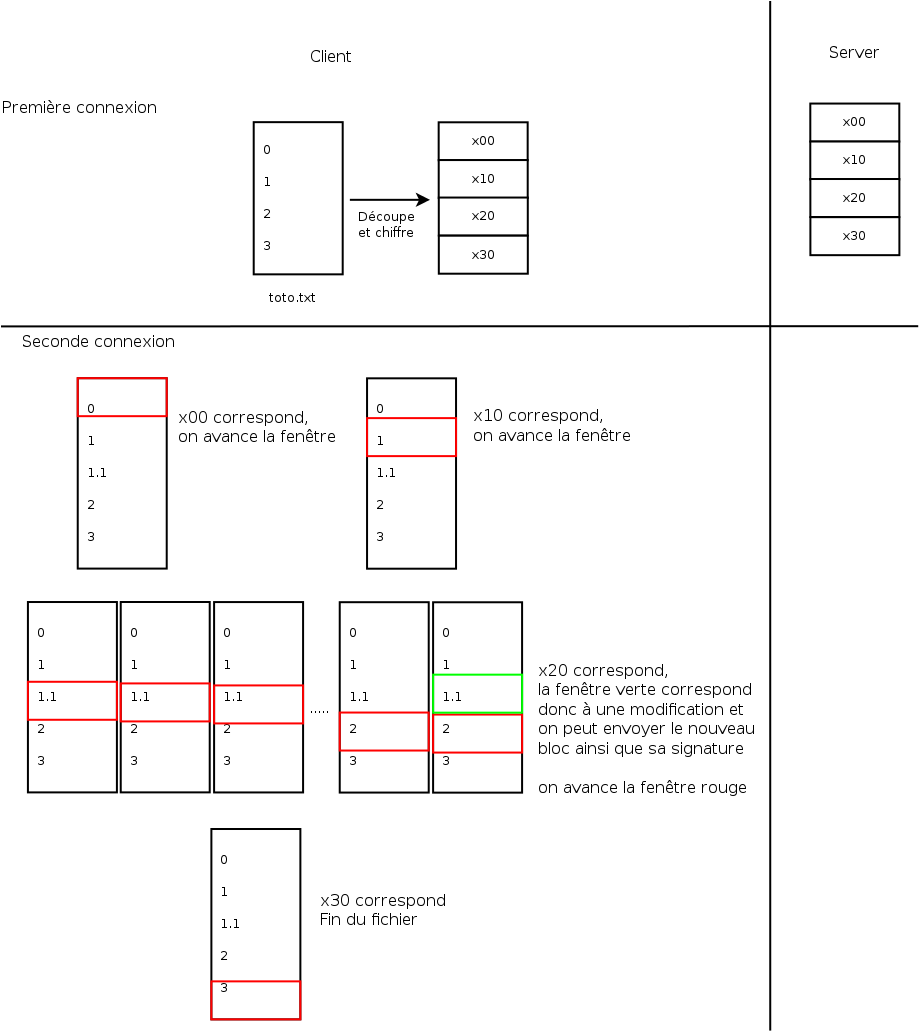
\includegraphics[width=15cm]{algo/rsyncalgo.png}
    \caption{\label{rsyncAlgo} Sch\'ema montrant bri\`evement
    l'algorithme \textit{rsync}}
\end{figure}

Celui-ci va d\'ecouper un fichier en plusieurs blocs de taille identique avant
de calculer, pour chacun, un \texttt{checksum} ainsi qu'un \texttt{hash}.

Pour n'envoyer que les parties modifi\'ees d'un ficher, l'algorithme va cr\'eer
une fen\^etre de la taille des blocs. Celle-ci va parcourir l'int\'egralit\'e
du fichier octet par octet.

Pour chaque position de la fen\^etre, le \texttt{checksum} --- rapide \`a
calculer mais dont le risque de collision est \'elev\'e --- est calcul\'e et
compar\'e au \texttt{checksum} d\'ej\`a calcul\'e au pr\'ec\'edent backup de
chaque bloc composant le fichier. Si un \textit{checksum} correspond, le
\texttt{hash} --- plus lent \`a calculer mais un risque de collision beaucoup
plus faible, selon l'algorithme utilis\'e --- du bloc correspondant est alors
comparer. Si celui-ci est identique, la fen\^etre correspond \`a un bloc non
modifi\'e du fichier.

Ainsi, tout ce qui pr\'ec\`ede la fen\^etre, et jusqu'au pr\'ec\'edent bloc
trouv\'e, correspondant \`a une partie du fichier modifi\'ee
(ajout/modification/suppression) et doit donc \^etre synchronis\'e.

C'est en grande partie cet algorithme qui m'a permis d'en trouver me permettant
de r\'epondre \`a ma probl\'ematique. Probl\'ematique \`a la fois similaire au
probl\`eme de \textit{rsync} puisqu'il fallait comparer deux fichiers distant
pour n'envoyer les changements mais diff\'erent dans la mesure o\`u il n'est
pas possible dans mon cas de maintenir une liste de bloc de m\^eme taille au
del\`a du premier backup.

\subsubsection{R\'eflexion}
Une fois cette phase de documentation r\'ealis\'ee, il \'etait temps de trouver
un algorithme permettant d'identifier les parties d'un fichier ayant \'et\'e
modifi\'e depuis le pr\'ec\'edent backup. Pour ce faire, et comme indiqu\'e
dans la partie documentation, je me suis bas\'e sur l'algorithme \textit{rsync}
pour, petit \`a petit, cr\'eer un algorithme qui permettait de r\'epondre \`a ma
probl\'ematique.

\paragraph{Chiffrement homomorphe\\}
Dans un premier temps, j'ai \'etudi\'e la question de l'homomorphisme. Ce type
de chiffrement permet de r\'ealiser des op\'erations sur des fichiers chiffr\'es
et de retourner le r\'esultat chiffr\'e. Ceci permet de faire des op\'erations
sans avoir \`a conna\^itre le contenu d'un fichier.

\begin{itemize}
 \item \textbf{Fonctionnement :} Dans notre cas, il nous aurait permis de concatener
 sur le serveur l'ensemble des morceaux d'un fichier avant de le re-d\'ecouper
 en bloc de taille \'egale puis de calculer pour chacun le \texttt{checksum}
 ainsi que le \texttt{hash}. Ceci aurait permis d'utiliser directement
 l'algorithme \textit{rsync} pour identifier les modifications faites sur un
 fichier.

 \item \textbf{Avantage :} Consommation de ressource et temps de calcul r\'eduit sur
 la machine client.
 
 \item \textbf{Inconv\'enient :} En utilisant le chiffrement homomorphe, le plus gros
 du calcul se fait sur le serveur entre deux backup, et ceux pour chaque
 fichier de chaque utilisateur. Ce type de chiffrement est donc tr\`es
 demandeur de ressource du c\^ot\'e du serveur pour que le programme fonctionne
 correctement.

 \item \textbf{Probl\`eme :} Le chiffrement homomorphe est un domaine de recherche
 tr\`es prometteur mais pas encore assez avanc\'e pour pouvoir \^etre utilis\'e
 en production. De plus le temps de calcul est extr\^emement \'elev\'e. Cette
 solution ne peut donc pas \^etre utilis\'ee aujourd'hui mais pourra peut-\^etre
 un jour \^etre envisag\'ee dans une prochaine version du backup.
\end{itemize}

\paragraph{rsync revisit\'e\\}
Ne pouvant rien faire du c\^ot\'e serveur, il fallait trouver un algorithme
qui permette de d'analyser un fichier en un temps fini. Pour cela, j'ai
travaill\'e \`a partir de l'id\'ee de fen\^etr glissante utilis\'ee pour
\textit{rsync}. Ne pouvant pas avoir des morceaux de fichier de taille
identique, il a fallu modifier l'algorithme pour prendre ceci en compte. Ainsi
avoir une fen\^etre dynamique semblait \^etre l'option \`a prendre.

\begin{itemize}
 \item \textbf{Fonctionnement :} L'algorithme utilise une fen\^etre dynamique,
 parcourant l'int\'egralit\'e du fichier et adaptant sa taille en fonction
 des longueurs des morceaux de fichier que nous avons.
 
 \item \textbf{Avantage :} Fait c\^ot\'e client, il n'y a pas une sur-utilisation
 des ressources serveurs qui est alors utilis\'e uniquement pour stocker
 les donn\'ees une fois chiffr\'ees.
 
 \item \textbf{Inconv\'enient :} Temps de calcul potentiellement grand, d\'ependant
 de la taille des fichiers \`a analyser ainsi que de ressources disponible sur
 la machine client.
\end{itemize}

C'est donc sur cette base que j'ai commenc\'e l'\'etape suivante. \'Etape 
consistant \`a \'ecrire un prototype permettant de v\'erifier la faisabilit\'e,
notamment en ce qui concerne le temps d'ex\'ecution du programme.

\subsubsection{Prototypage}
La v\'erification pratique de la th\'eorie \'etait n\'ecessaire avant de
pouvoir penser \`a la conception du produit. Pour cela, le passage par une
\'etape de prototypage semblait in\'evitable.

Dans ce cadre, j'ai \'ecrit l'algorithme en \textit{C++} afin de v\'erifier
le temps d'ex\'ecution de celui-ci. Plusieurs essais ont \'et\'e fait afin de
r\'eduire toujours plus la dur\'ee d'ex\'ecution de l'algorithme. C'est donc
principalement de l'optimisation, \`a la fois au niveau algorithmique ainsi
qu'au niveau de l'\'ecriture du code en lui-m\^eme, que j'ai effectu\'e  au
course de cette \'etape.

Plusieurs version ont donc vu le jour au cours de cette \'etape afin d'obtenir
un algorithme qui puisse \^etre utilisable pour le syst\`eme de backup.

Plus de d\'etails sur ces diff\'erentes versions de l'algorithme peuvent \^etre
trouv\'es dans la partie~\nameref{rapportTechnique}.


\subsection{Conception}
\subsection{D\'eveloppement}

\chapter{Rapport technique}
\thispagestyle{fancy}
\label{rapportTechnique}
\subsection{Travail de recherche}
\subsubsection{Prototypage}
Comme expliqu\'e dans le~\nameref{rapportSynthese}, une v\'erification pratique
de la faisabilit\'e de l'algorithme choisi \'etait n\'ecessaire avant de
pouvoir entamer la conception du produit et plusieurs versions on vu le jour.

\paragraph{Premi\`ere version}



\newpage
\listoffigures
\listoftables
\bibliographystyle{abbrv-fr}
\bibliography{rapport_stage_arksens_2015}

\end{spacing}
\end{document}          